% Quantum Imaginary-Time Evolution (QITE): study notes for the Quantinuum QITE-vs-Krylov benchmark.
% Exploration log: entries are appended, never deleted.
% Build:  ../tools/build-tex.sh quantum-imaginary-time-evolution.tex
\documentclass[11pt,a4paper]{article}
\usepackage{mathnotes}

% Local (topic-only) notation -- kept here so the shared mathnotes.sty is untouched.
\newcommand{\ket}[1]{\lvert #1\rangle}
\newcommand{\bra}[1]{\langle #1\rvert}
\newcommand{\braket}[2]{\langle #1\vert #2\rangle}
\newcommand{\expect}[1]{\langle #1\rangle}
\newcommand{\Htil}{\widetilde H}
\graphicspath{{../figures/}}

\title{Quantum Imaginary-Time Evolution (QITE)\\\large Study notes and benchmark plan against Quantum Krylov}
\author{Prajjwal}
\date{Started 2026-10-08 \\ \small Last built: \today}

\begin{document}
\maketitle
\tableofcontents
\bigskip

%=====================================================================================
\entry{2026-10-08}{QITE from first principles}

\begin{question}
Prepare very good notes on Quantum Imaginary-Time Evolution (QITE): why imaginary time finds
the ground state, why $e^{-\tau H}$ cannot be run directly as a circuit, how QITE replaces it
by a unitary $e^{-i\Delta\tau A}$ with $A$ determined from measured expectation values, how it
compares with Quantum Krylov, and how to benchmark both on Quantinuum hardware for the
molecular ground-state energy (e.g.\ $\mathrm{H}_2$).
\end{question}

\paragraph{Reading guide.}
\Cref{sec:why,sec:nonunitary} are the physics. \Cref{sec:qite} is the algorithm and its
derivation, the part to master. \Cref{sec:cost} is cost and pitfalls, \cref{sec:krylov}
the comparison with Krylov. The numerical check on $\mathrm{H}_2$ is in
\cref{sec:numerics} and the experimental design in \cref{sec:bench}. Throughout,
$H=\sum_{m}h_m P_m$ is a qubit Hamiltonian with Pauli strings $P_m$, $\hbar=1$, and energies
in Hartree.

%-------------------------------------------------------------------------------------
\subsection{Why imaginary time finds the ground state}\label{sec:why}

Let $H\ket{E_n}=E_n\ket{E_n}$ with $E_0<E_1\le E_2\le\cdots$ and write the initial state as
$\ket{\psi_0}=\sum_n c_n\ket{E_n}$. Replace real time $e^{-iHt}$ by imaginary time
$t=-i\tau$:
\begin{equation}
  \ket{\psi(\tau)}=\frac{e^{-\tau H}\ket{\psi_0}}{\norm{e^{-\tau H}\ket{\psi_0}}},
  \qquad
  e^{-\tau H}\ket{\psi_0}=e^{-\tau E_0}\Big[c_0\ket{E_0}+\sum_{n>0}c_n e^{-\tau(E_n-E_0)}\ket{E_n}\Big].
\end{equation}

\begin{proposition}[Convergence]\label{prop:conv}
If $c_0\neq0$ and $\Delta=E_1-E_0>0$ is the gap, then $\ket{\psi(\tau)}\to\ket{E_0}$ and
\begin{equation}
  E(\tau)-E_0 \;\le\; \frac{\sum_{n>0}\abs{c_n}^2 (E_n-E_0)\,e^{-2\tau(E_n-E_0)}}{\abs{c_0}^2}
  \;=\;O\!\big(e^{-2\tau\Delta}\big),
  \qquad E(\tau)=\frac{\bra{\psi(\tau)}H\ket{\psi(\tau)}}{\braket{\psi(\tau)}{\psi(\tau)}}.
\end{equation}
\end{proposition}
\begin{proof}
$E(\tau)-E_0=\sum_n \abs{c_n}^2e^{-2\tau(E_n-E_0)}(E_n-E_0)\big/\sum_n\abs{c_n}^2e^{-2\tau(E_n-E_0)}$.
The denominator is at least $\abs{c_0}^2$, giving the bound.
\end{proof}

\begin{remark}
Two things control the rate: the gap $\Delta$ (a small gap needs a long $\tau$) and the
overlap $\abs{c_0}^2$ (the prefactor). Hartree--Fock typically has $\abs{c_0}^2\approx0.9$+,
so the prefactor is benign and the \alert{gap} is the real cost driver. Only states in the
same symmetry sector as $\ket{\psi_0}$ matter: for $\mathrm{H}_2$ in \cref{sec:numerics} the
relevant gap is that of the $2\times2$ sector containing HF ($1.632$\,Ha), not the global
gap ($0.613$\,Ha).
\end{remark}

\begin{figure}[ht]\centering
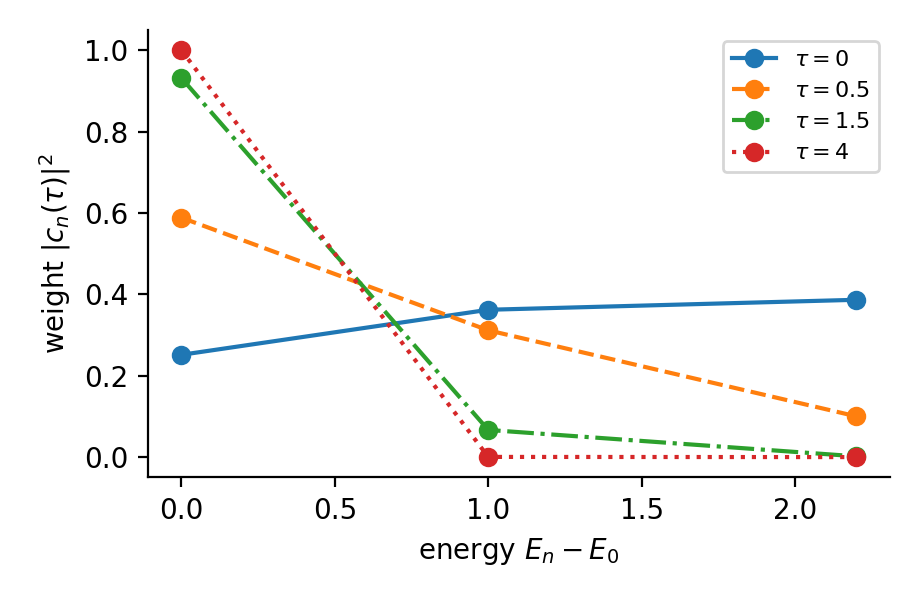
\includegraphics[width=.5\linewidth]{filter.png}
\caption{Imaginary-time evolution as a filter: weights $\abs{c_n(\tau)}^2$ on a toy
three-level spectrum. Excited weight decays as $e^{-2\tau(E_n-E_0)}$.}
\end{figure}

\subsubsection*{The normalised flow and the energy-descent law}
The normalised state obeys a nonlinear equation. Differentiating the quotient above,
\begin{equation}\label{eq:flow}
  \od{}{\tau}\ket{\psi}=-\big(H-E(\tau)\big)\ket{\psi}.
\end{equation}
The $E(\tau)$ term is exactly what keeps the norm fixed; the physical content is
$-H\ket\psi$ projected orthogonal to $\ket\psi$.

\begin{proposition}[Energy descent]\label{prop:descent}
Along \cref{eq:flow}, $\displaystyle\od{E}{\tau}=-2\Var_\psi(H)=-2\big(\expect{H^2}-\expect{H}^2\big)\le0$,
with equality iff $\ket\psi$ is an eigenstate.
\end{proposition}
\begin{proof}
$\od{E}{\tau}=2\operatorname{Re}\bra\psi H\ket{\dot\psi}
=-2\operatorname{Re}\bra\psi H(H-E)\ket\psi=-2(\expect{H^2}-E\expect H)=-2\Var_\psi(H)$.
\end{proof}

\begin{remark}[Diagnostic]
\Cref{prop:descent} is exact for ideal ITE. For QITE the measured $E$ should be (nearly)
monotone and $\Var_\psi(H)\to0$. An increasing energy signals approximation error
(domain too small, $\Delta\tau$ too large, ill-conditioned $S$) or shot noise/hardware noise.
The variance $\Var_\psi(H)$ is also a rigorous eigenstate certificate: some eigenvalue lies within
$\sqrt{\Var_\psi(H)}$ of $E(\tau)$.
\end{remark}

\begin{remark}[Power iteration]
$e^{-\tau H}$ is the continuous analogue of power iteration with the filter
$f(H)=e^{-\tau H}$ (equivalently $(\lambda_{\max}-H)^k$). This is why QITE and
Krylov methods are cousins: both are polynomial/filter approximations to a spectral projector.
\end{remark}

%-------------------------------------------------------------------------------------
\subsection{Why $e^{-\tau H}$ cannot simply be a circuit}\label{sec:nonunitary}

A circuit implements a unitary, $U^\dagger U=I$. But $e^{-\tau H}$ is Hermitian positive
definite with $(e^{-\tau H})^\dagger e^{-\tau H}=e^{-2\tau H}\neq I$ for any $\tau\neq0$ unless
$H\propto I$. It rescales each eigencomponent by $e^{-\tau E_n}$, so it changes both norm and
relative weights. (The statement ``$\abs{e^{-\tau E_n}}<1$'' only holds if $E_n>0$; the point is
that the factors are \emph{not of modulus one}.) The state after normalisation is physical,
but the map is not unitary.

There are three families of workarounds:
\begin{enumerate}
\item \key{Unitary surrogate (QITE, Motta et al.)}: find a Hermitian $A$ with
$e^{-i\Delta\tau A}\ket\psi\approx e^{-\Delta\tau H}\ket\psi/\sqrt c$ \emph{on the current state}.
\item \key{Variational (VarQITE, McLachlan)}: parametrise $\ket{\psi(\vec\theta)}$ and
propagate $\vec\theta$ by an ODE (\cref{sec:var}).
\item \key{Probabilistic/ancilla (block-encoding, LCU)}: embed $e^{-\tau H}$ in a larger unitary
and post-select; succeeds with probability $\sim\norm{e^{-\tau H}\ket\psi}^2$, which decays
exponentially in $\tau$. Not NISQ-friendly.
\end{enumerate}

%-------------------------------------------------------------------------------------
\subsection{The QITE algorithm}\label{sec:qite}

\subsubsection*{Step 1: Trotterise the Hamiltonian}
Write $H=\sum_{m=1}^{M}h_m$ with each $h_m$ a \emph{local} Pauli term (coefficient times
Pauli string, possibly grouped). To first order in $\Delta\tau$,
\begin{equation}\label{eq:trot}
  e^{-\Delta\tau H}=\prod_{m=1}^M e^{-\Delta\tau h_m}+O(\Delta\tau^2).
\end{equation}
Each factor $e^{-\Delta\tau h_m}$ acts on few qubits, which is what makes a local unitary
surrogate plausible. For $h_m=\alpha_m P_m$ with $P_m^2=I$,
$e^{-\Delta\tau h_m}=\cosh(\Delta\tau\alpha_m)I-\sinh(\Delta\tau\alpha_m)P_m$.

\subsubsection*{Step 2: One local step}
Given the current normalised state $\ket{\psi}$, define the target
\begin{equation}
  \ket{\psi'}=\frac{e^{-\Delta\tau h_m}\ket\psi}{\sqrt{c_m}},\qquad
  c_m=\bra\psi e^{-2\Delta\tau h_m}\ket\psi=1-2\Delta\tau\expect{h_m}+O(\Delta\tau^2).
\end{equation}
We want a Hermitian $A_m=\sum_{\mu\in\mathcal D_m}a_\mu\sigma_\mu$, with $\sigma_\mu$ Pauli strings
in a domain $\mathcal D_m$ (typically all strings on the qubits within distance $D$ of the support of $h_m$), such that
$e^{-i\Delta\tau A_m}\ket\psi\approx\ket{\psi'}$. Expanding to first order,
$e^{-i\Delta\tau A_m}\ket\psi\approx\ket\psi-i\Delta\tau A_m\ket\psi$, so we need
\begin{equation}
  -iA_m\ket\psi\approx\ket{d}\defeq\frac{\ket{\psi'}-\ket\psi}{\Delta\tau}.
\end{equation}

\begin{proposition}[Linear system for $\vec a$]\label{prop:linsys}
Minimising $\norm{-iA_m\ket\psi-\ket d}^2$ over real $\vec a$ gives
\begin{equation}\label{eq:linsys}
  \boxed{\;S\vec a=\vec b,\qquad
  S_{\mu\nu}=\operatorname{Re}\bra\psi\sigma_\mu\sigma_\nu\ket\psi,\qquad
  b_\mu=-\operatorname{Im}\bra\psi\sigma_\mu\ket{d}\;}
\end{equation}
\end{proposition}
\begin{proof}
The cost is $f(\vec a)=\norm{\sum_\nu a_\nu(-i\sigma_\nu\ket\psi)-\ket d}^2$. Setting
$\pd{f}{a_\mu}=0$ gives $\sum_\nu a_\nu\operatorname{Re}\langle -i\sigma_\mu\psi\vert -i\sigma_\nu\psi\rangle
=\operatorname{Re}\langle -i\sigma_\mu\psi\vert d\rangle$. Now
$\langle\sigma_\mu\psi\vert\sigma_\nu\psi\rangle=\bra\psi\sigma_\mu\sigma_\nu\ket\psi$
and $\operatorname{Re}(i\bra\psi\sigma_\mu\ket d)=-\operatorname{Im}\bra\psi\sigma_\mu\ket d$.
\end{proof}

\paragraph{Everything is a measurement.}
$S_{\mu\nu}$ is the expectation of the Pauli string $\sigma_\mu\sigma_\nu$ (a Pauli up to a phase),
estimated by measuring on the current circuit $U_{k}\cdots U_1\ket{\psi_0}$. For $\vec b$,
substitute $\ket d$:
\begin{equation}
  b_\mu=-\frac{1}{\Delta\tau}\operatorname{Im}\Big[\tfrac{1}{\sqrt{c_m}}\bra\psi\sigma_\mu e^{-\Delta\tau h_m}\ket\psi-\bra\psi\sigma_\mu\ket\psi\Big],
  \qquad e^{-\Delta\tau h_m}=\cosh(\Delta\tau\alpha_m)-\sinh(\Delta\tau\alpha_m)P_m,
\end{equation}
and $\bra\psi\sigma_\mu\ket\psi$ is real (Hermitian Pauli), so only the $\sigma_\mu P_m$ term survives:
\begin{equation}
  b_\mu=\frac{\sinh(\Delta\tau\alpha_m)}{\Delta\tau\sqrt{c_m}}\operatorname{Im}\bra\psi\sigma_\mu P_m\ket\psi .
\end{equation}
Since $\sigma_\mu P_m$ is $\pm i$ times a Hermitian Pauli whenever $\sigma_\mu,P_m$ anticommute
(and Hermitian when they commute), $b_\mu$ is nonzero only for \emph{anticommuting} pairs:
each is a single Pauli expectation. No ancillas, no Hadamard tests, only basis rotations and
computational-basis measurement. This is the key practical feature.

\paragraph{Real structure.}
For a real Hamiltonian and a real initial state ($\mathrm{H}_2$, HF) the state stays real,
$\bra\psi\sigma_\mu\ket\psi=0$ when $\sigma_\mu$ has an even number of $Y$, and $S$ restricted to
strings with an \emph{odd} number of $Y$ is the relevant block. This halves the domain.

\subsubsection*{Step 3: Implement the unitary}
The step operator is $e^{-i\Delta\tau A_m}$ with $A_m=\sum_\mu a_\mu\sigma_\mu$; the strings in
$A_m$ do not commute, so one Trotterises again,
$e^{-i\Delta\tau A_m}\approx\prod_\mu e^{-i\Delta\tau a_\mu\sigma_\mu}$, each factor a Pauli
rotation (CNOT ladder around one $R_z$, or native $ZZ$-type phase gates on trapped-ion
hardware). Then set $\ket\psi\leftarrow e^{-i\Delta\tau A_m}\ket\psi$ and move to $m+1$.

\paragraph{Algorithm (one pass over $M$ terms = one imaginary-time step $\Delta\tau$).}
\begin{enumerate}
\item Prepare $\ket{\psi}=U_k\cdots U_1\ket{\psi_0}$ (all previous step unitaries).
\item For $m=1,\dots,M$:
  \begin{enumerate}
  \item Choose the domain $\mathcal D_m$ (size $D$, $d_m=\lvert\mathcal D_m\rvert$ Pauli strings).
  \item Measure $\expect{h_m}$ (for $c_m$), all $S_{\mu\nu}$, all $b_\mu$.
  \item Solve $S\vec a=\vec b$ (regularised, least squares).
  \item Append $U_{k+1}=e^{-i\Delta\tau\sum_\mu a_\mu\sigma_\mu}$ to the circuit.
  \end{enumerate}
\item Measure $E=\expect H$ (and $\Var H$); stop when converged, else repeat.
\end{enumerate}

\begin{remark}[Correction to a common simplification]
It is tempting to describe QITE as ``repeatedly executing relatively shallow circuits
$U_1,\dots,U_K$''. Each $U_j$ is shallow, but the state at step $k$ is $U_k\cdots U_1\ket{\psi_0}$: the
circuit depth \alert{grows linearly with the number of steps}, and one cannot reuse the previous
state without re-preparing it. Depth per step is small; total depth is not. This is the main
difference from a fixed-depth VQE ansatz and is what the benchmark must measure honestly
(\cref{sec:cost}).
\end{remark}

\subsubsection*{Locality and the size of the domain}
Why should a local $A_m$ exist at all? If the state has finite correlation length $\xi$, then
$e^{-\Delta\tau h_m}\ket\psi$ differs from $\ket\psi$ only by a quasi-local perturbation, and
Motta et al.\ show the approximation error decays with the domain size roughly as $e^{-D/\xi}$,
whereas the number of strings grows as $4^{D}$ (per dimension-dependent volume). For a general
molecule, where interactions are not geometrically local after a fermion-to-qubit map, the useful
domain can be \alert{all} $4^{N_q}$ strings, which is exponential. For $\mathrm{H}_2$ (2 qubits) the full
domain is just 16 (or 6 odd-$Y$) strings, which is why it is an easy test case and also why it is
\alert{not} representative of scaling.

\subsubsection*{Imaginary time $\leftrightarrow$ unitary: what is exact}
With $\mathcal D$ the full Pauli group the equation $-iA\ket\psi=\ket d$ has an exact solution
(for any two non-orthogonal states there is a Hermitian generator mapping one to the other), so the
only remaining errors are the \emph{first-order expansion} in $\Delta\tau$, the Trotter splitting
\cref{eq:trot} and the \emph{conditioning} of $S$. Truncating $\mathcal D$ adds a systematic
error on top.

%-------------------------------------------------------------------------------------
\subsection{Variational QITE (McLachlan) and relations}\label{sec:var}
Take an ansatz $\ket{\psi(\vec\theta)}$ and impose the McLachlan principle
$\delta\norm{(\partial_\tau+H-E)\ket\psi}=0$, giving
\begin{equation}
  \sum_j M_{ij}\dot\theta_j=-C_i,\qquad
  M_{ij}=\operatorname{Re}\langle\partial_i\psi\vert\partial_j\psi\rangle,\quad
  C_i=\tfrac12\partial_i E .
\end{equation}
$M$ is the quantum geometric tensor (Fubini--Study metric up to normalisation and the
$\langle\partial_i\psi\vert\psi\rangle$ terms) so VarQITE is \key{natural gradient descent} on $E(\vec\theta)$. Differences from
QITE: fixed circuit depth (set by the ansatz) but an \emph{ansatz-expressibility} error and
possible local minima; QITE has no ansatz, but its depth grows. If one writes the QITE
generator $A$ as a parameter of an ever-growing ansatz, QITE is the same linear system with a
growing parameter set.

%-------------------------------------------------------------------------------------
\subsection{Cost, conditioning and pitfalls}\label{sec:cost}

\paragraph{Per step.}
With $M$ terms and domain size $d$ per term the number of distinct Pauli expectation values is
$O(M d^2)$ for $S$ and $O(M d)$ for $\vec b$ (many repeated). Each must be estimated to
precision $\epsilon$, costing $O(1/\epsilon^2)$ shots, grouped by qubit-wise commuting
measurement bases.

\paragraph{Circuit growth.}
After $N$ steps there are $\sim NM$ unitaries each with up to $d$ Pauli rotations:
\begin{equation}
  \text{depth}\;\sim\;N\cdot M\cdot d\cdot (\text{depth of one Pauli rotation}),\qquad
  N_{2q}\;\sim\;N M d\,\bar w,
\end{equation}
$\bar w$ being the mean weight of the strings. The number of circuits executed to reach
step $N$ is $\sim\sum_{k\le N}(\text{measurement settings}\;\cdot\text{shots})$, i.e.\ quadratic in $N$ if
circuit lengths grow linearly and one pays for the whole prefix at every step.

\paragraph{Ill-conditioning.}
Near convergence, $\sigma_\mu\ket\psi$ become nearly linearly dependent (indeed
$\ket\psi\to$ eigenstate, so $A\ket\psi\to$ small, and many strings give the same vector):
$S$ becomes \alert{singular}. With shot noise, $\vec a=S^{-1}\vec b$ amplifies the noise by $\kappa(S)$.
Standard remedies: Tikhonov $S+\epsilon I$, truncated SVD / pseudo-inverse, or a larger
$\Delta\tau$ so $\vec b$ is not tiny relative to the noise. This is the QITE analogue of the
overlap-matrix thresholding in Krylov.

\paragraph{Summary table of pitfalls.}
\begin{center}
\small\begin{tabular}{@{}p{3cm}p{4.8cm}p{5.4cm}@{}}
\toprule
Source & Effect & Mitigation\\
\midrule
$\Delta\tau$ too large & Trotter and first-order error, energy plateau above $E_0$ & Halve $\Delta\tau$; second-order splitting\\
$\Delta\tau$ too small & Many steps, deep circuit, noise accumulates & Choose $\Delta\tau\sim0.1$--$0.5/\norm H$ scale; adaptive\\
Small domain & Systematic bias, may stall & Grow $D$; check against exact for small $N_q$\\
Ill-conditioned $S$ & Noise amplification, energy drifts up & Regularise, SVD cut-off, more shots\\
Hardware noise & Mixed state, $E$ above the ideal curve & Error mitigation; compare on identical noise model\\
Symmetry sector & Wrong state if $\ket{\psi_0}$ has no $c_0$ & Initialise in the right $(N,S_z)$ sector\\
\bottomrule
\end{tabular}
\end{center}

%-------------------------------------------------------------------------------------
\subsection{QITE versus Quantum Krylov}\label{sec:krylov}

Quantum Krylov (QKSD / filter diagonalisation) prepares states
$\ket{\phi_j}=e^{-iHt_j}\ket{\psi_0}$ ($j=0,\dots,K-1$; commonly $t_j=j\,\delta t$), measures
\begin{equation}
  H_{jk}=\bra{\phi_j}H\ket{\phi_k},\qquad S_{jk}=\braket{\phi_j}{\phi_k},
\end{equation}
by Hadamard-type or time-shifted-overlap circuits, and solves the generalised eigenproblem
$HC=ESC$. For real-time evolution with equally spaced times both matrices are Toeplitz-like:
$S_{jk}=s(t_k-t_j)$, so only $\sim 2K$ distinct overlaps are required.

\begin{center}
\small\begin{tabular}{@{}p{2.6cm}p{5.2cm}p{5.2cm}@{}}
\toprule
 & Quantum Krylov & QITE\\
\midrule
Quantum part & Overlaps $\bra{\psi_0}e^{-iHt}\ket{\psi_0}$ and $\bra{\psi_0}He^{-iHt}\ket{\psi_0}$ (Hadamard test or equivalents) & Pauli expectation values $S_{\mu\nu},b_\mu$ at every step\\
Classical part & One small generalised eigenproblem & A least-squares solve per term per step\\
Circuit per run & Time evolution $e^{-iHt}$ (Trotter), depth $\propto t$, \emph{fixed per $K$} & Prefix grows with step number\\
Error source & Trotter error in $e^{-iHt}$; $S$ ill-conditioning when $\delta t$ small or $K$ large & Domain truncation, first-order $\Delta\tau$, $S$ ill-conditioning\\
Convergence & Subspace error $\sim$ Chebyshev-like in $K$; independent of a step schedule & $e^{-2\tau\Delta}$ at best\\
Noise robustness & Overlap noise enters the generalised eigenproblem; thresholding required & Noise enters each step and is \emph{accumulated} in the state\\
Qubits & $N_q$ (+1 ancilla for Hadamard test) & $N_q$\\
\bottomrule
\end{tabular}
\end{center}

\begin{remark}[Why they are cousins]
Real-time Krylov with $t_j=j\,\delta t$ spans $\{p(e^{-iH\delta t})\ket{\psi_0}\}$ over polynomials of
degree $<K$; QITE applies one specific filter $e^{-\tau H}$. Krylov \emph{optimises} the filter
(Rayleigh--Ritz picks the best combination in the span), so for a given number of applications of
the propagator it can converge faster than a fixed filter, but needs the classical post-processing
and robust $S$. QITE has no such optimisation, but needs no overlap circuits.
\end{remark}

%=====================================================================================
\entry{2026-10-08}{Numerical check on $\mathrm{H}_2$}\label{sec:numerics}

\begin{question}
Implement QITE for the 2-qubit $\mathrm{H}_2$ Hamiltonian, compare with exact ITE and a small
Quantum Krylov baseline, and quantify the effect of shot noise.
\end{question}

\paragraph{Setup.}
$\mathrm{H}_2$, STO-3G, $R=0.735$\,\AA, parity mapping with two-qubit reduction
(the standard 2-qubit Hamiltonian; nuclear repulsion $0.7200$\,Ha excluded):
\begin{equation}
  H=-1.0524\,II+0.3979\,IZ-0.3979\,ZI-0.0113\,ZZ+0.1809\,XX .
\end{equation}
Exact diagonalisation: $E_{\rm FCI}=-1.857275$\,Ha; Hartree--Fock (the basis state $\ket{01}$)
$-1.836968$\,Ha, i.e.\ a correlation energy of $20.3$\,mHa; $\abs{c_0}^2=0.9877$.
Code: \texttt{code/qite\_h2.py}, run in \texttt{aq-env}. QITE uses the full odd-$Y$ domain
$\{IY,XY,YI,YX,YZ,ZY\}$, $\Delta\tau=0.1$, 60 steps, one first-order Trotter pass per step,
regularisation $10^{-6}$. Krylov uses real time $\delta t=0.5$ with an exact propagator
(this isolates the subspace error; Trotter error is not included). Shot noise is emulated by adding
Gaussian noise of size $1/\sqrt{N_{\rm shots}}$ to every entry of $S$ and $\vec b$ (a crude model,
independent per entry and ignoring the shot cost of grouping).

\begin{figure}[ht]\centering
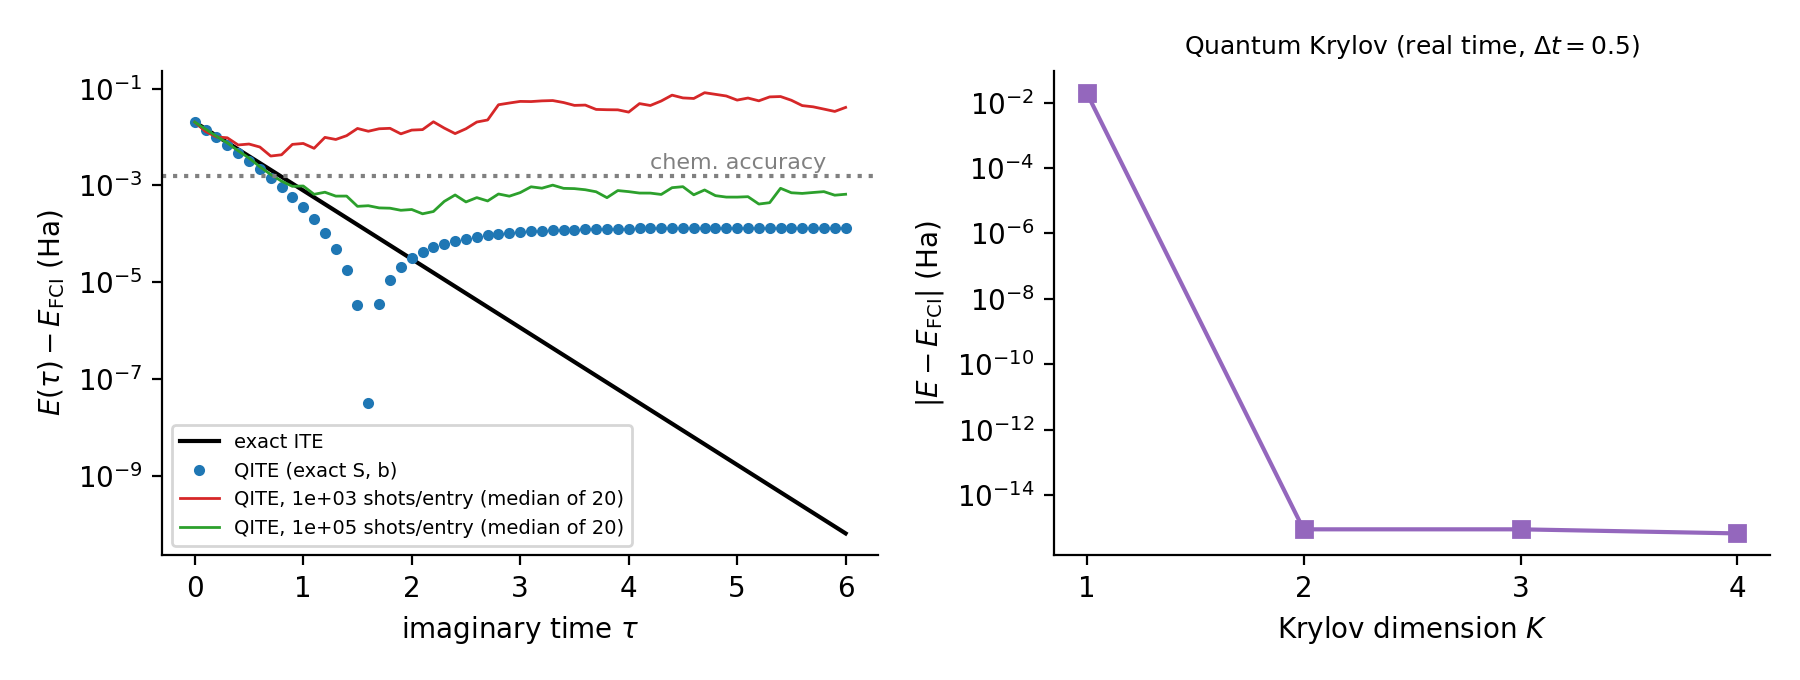
\includegraphics[width=\linewidth]{h2_convergence.png}
\caption{Left: energy error versus imaginary time for exact ITE, QITE with exactly evaluated $S,\vec b$,
and QITE with shot-noisy $S,\vec b$ (median of 20 seeds). Right: Quantum Krylov versus subspace dimension.}
\end{figure}

\begin{center}
\small\begin{tabular}{@{}p{8.2cm}p{7cm}@{}}
\toprule
Quantity & Value\\
\midrule
Steps to chemical accuracy (1.6\,mHa), exact ITE / QITE & 8 / 7\\
Final error, exact ITE ($\tau=6$) & $\sim10^{-10}$ Ha\\
Best / final error, QITE (exact $S,\vec b$) & $3\times10^{-8}$ ($\tau=1.6$) / $1.3\times10^{-4}$ Ha\\
Plateau error, QITE, $10^{3}$ shots/entry (mean over 20 seeds) & $0.15$ Ha\\
Plateau error, QITE, $10^{5}$ shots/entry & $2.0\times10^{-3}$ Ha\\
Quantum Krylov error, $K=1,2,3,4$ & $2.0\times10^{-2}$, $<10^{-14}$, $<10^{-14}$, $<10^{-14}$ Ha\\
\bottomrule
\end{tabular}
\end{center}

\paragraph{Conclusions.}
\begin{enumerate}
\item With exact $S,\vec b$ QITE reproduces exact ITE down to chemical accuracy in a few steps,
confirming the derivation in \cref{prop:linsys}.
\item The QITE energy is \alert{not monotone}: it reaches an error of $3\times10^{-8}$\,Ha at $\tau=1.6$ and then
\emph{drifts back up} to a plateau at $\approx1.3\times10^{-4}$\,Ha, whereas exact ITE keeps decaying. This is
the singularity of $S$ near the ground state discussed in \cref{sec:cost}, interacting with the
regularisation and the first-order step; it violates \cref{prop:descent} and is exactly the symptom the
variance diagnostic should flag. Energies stayed above $E_{\rm FCI}$ (variational), as they must.
\item Shot noise is far more damaging than the algorithm error: at $10^3$ shots per matrix entry
the result is worse than the starting HF point (error $0.15$\,Ha $>$ HF error $0.020$\,Ha) because noisy
$S$ is inverted. At $10^5$ shots the plateau is roughly chemical accuracy. This is the quantitative
form of ``QITE needs many measurements''.
\item Quantum Krylov is exact at $K=2$ here only because the HF state lives in a $2\times2$ symmetry
sector, so any 2-dimensional Krylov space spans it. \alert{$\mathrm{H}_2$ cannot discriminate the two methods}:
it is a test of correctness, not of scaling. A discriminating benchmark needs $\ge4$ qubits
(e.g.\ $\mathrm{LiH}$ active space, $\mathrm{H}_4$) where the sector is large.
\end{enumerate}

%=====================================================================================
\entry{2026-10-08}{Benchmark design on Quantinuum hardware}\label{sec:bench}

\begin{question}
Under identical Quantinuum resource constraints, how do QITE and Quantum Krylov trade
accuracy, circuit depth, number of measurements and robustness?
\end{question}

\paragraph{Metrics (record all, per method and per budget point).}
\begin{center}
\small\begin{tabular}{@{}p{2.6cm}p{12.6cm}@{}}
\toprule
Metric & Definition\\
\midrule
Accuracy & $\abs{E-E_{\rm FCI}}$ in Ha and mHa; also $\Var_\psi(H)$ where available\\
Shots & total $N_{\rm shots}$ summed over \emph{all} circuits, including those for $S$, $H$-matrix, $\vec b$\\
Circuits & number of distinct circuit executions $N_{\rm circ}$ (after grouping)\\
Depth & maximum circuit depth $D$ over the run (QITE: last step; Krylov: deepest $e^{-iHt}$)\\
2-qubit gates & $N_{2q}$ per circuit and in total\\
Qubits & $N_q$ (+ancilla)\\
Wall time & $T$; for hardware also queue time and compile time reported separately\\
\bottomrule
\end{tabular}
\end{center}

\paragraph{Experiments.}
\begin{description}
\item[A. Ideal simulation] Noiseless statevector for both methods vs.\ $E_{\rm FCI}$; checks the code and
Trotter/domain errors alone.
\item[B. Noisy simulation] One \emph{shared} noise model (depolarising $2q$ rate, readout error,
finite shots) for both; separates algorithmic from hardware error.
\item[C. Hardware] Both on the same Quantinuum device/emulator, same date, same compiler settings.
\item[D. Budget-normalised] Fix $N_{\rm shots}$ and/or $N_{2q}$; compare accuracy at equal cost.
\item[E. Scaling curve] Vary $K$ (Krylov) and number of QITE steps $N$; plot
$\abs{E-E_{\rm FCI}}$ against hardware cost (shots, or $N_{2q}$ total). This is the central figure.
\end{description}

\paragraph{Fair-comparison rules.}
\begin{enumerate}
\item Same initial state (HF), same qubit mapping/tapering, same Hamiltonian grouping.
\item Count \emph{every} circuit run, including repeated prefixes in QITE and Hadamard-test ancillas
in Krylov.
\item Tune hyperparameters ($\Delta\tau$, domain, regularisation; $\delta t$, $K$, threshold) on
the noisy \emph{simulator}, then freeze them before hardware.
\item Report seeds / repeated runs: with shot noise a single curve is not evidence (cf.\ the 20-seed median above).
\item Always include the plain baselines: HF energy and VQE (or fixed-ansatz) at the same budget.
\end{enumerate}

\paragraph{Hypotheses to test (not results).}
\begin{itemize}
\item QITE has shallow per-step circuits but total depth growing with step count; it may win at small
budgets and lose when the prefix grows.
\item Krylov needs deeper $e^{-iHt}$ with fewer total repetitions but is sensitive to overlap noise;
the generalised eigenproblem may fail when $S$ is noisy.
\item Which wins on Quantinuum (high-fidelity, all-to-all two-qubit gates, mid-circuit
measurement) is empirical. Trapped-ion connectivity favours QITE's non-local Pauli rotations,
since no SWAP overhead is incurred, which removes one common penalty for large domains.
\end{itemize}

\paragraph{Open items.}
\todo{Confirm with the colleague which Krylov variant (real-time vs.\ filtered, Hadamard test vs.\ overlap-only) and which time grid $t_j$.}
\todo{Get the actual molecule, basis, active space, qubit mapping and Quantinuum target (device vs.\ emulator) before fixing the noise model.}
\todo{Extend \texttt{qite\_h2.py} to $N_q\ge4$ (e.g.\ LiH active space) with a locality-truncated domain, plus a Trotterised Krylov baseline.}

%=====================================================================================
\entry{2026-10-08}{Quick reference and references}

\paragraph{Formula sheet.}
\begin{align*}
  \text{ITE:}\quad & \ket{\psi(\tau)}\propto e^{-\tau H}\ket{\psi_0}, \quad \dot{\ket\psi}=-(H-E)\ket\psi,\quad \dot E=-2\Var_\psi H\\
  \text{Trotter:}\quad & e^{-\Delta\tau H}\approx\textstyle\prod_m e^{-\Delta\tau h_m}\\
  \text{Surrogate:}\quad & e^{-\Delta\tau h_m}\ket\psi/\sqrt{c_m}\approx e^{-i\Delta\tau A_m}\ket\psi,\ A_m=\textstyle\sum_\mu a_\mu\sigma_\mu\\
  \text{Linear system:}\quad & S_{\mu\nu}=\operatorname{Re}\expect{\sigma_\mu\sigma_\nu},\ b_\mu=\tfrac{\sinh(\Delta\tau\alpha_m)}{\Delta\tau\sqrt{c_m}}\operatorname{Im}\expect{\sigma_\mu P_m}\\
  \text{Krylov:}\quad & HC=ESC,\ S_{jk}=\braket{\phi_j}{\phi_k},\ \ket{\phi_j}=e^{-iHt_j}\ket{\psi_0}
\end{align*}

\paragraph{Self-test questions.}
\begin{enumerate}
\item Why is $b_\mu=0$ when $\sigma_\mu$ commutes with $P_m$?
\item Why does $S$ become singular as $\ket\psi\to\ket{E_0}$, and what does regularisation trade away?
\item Show that the McLachlan equation with a rotation ansatz reproduces \cref{eq:linsys}.
\item Which gap controls convergence for a state in a given symmetry sector?
\end{enumerate}

\paragraph{References} (quoted from memory; check details before citing).
\begin{itemize}
\item M.~Motta et al., ``Determining eigenstates and thermal states on a quantum computer using quantum imaginary time evolution'', \emph{Nature Physics} \textbf{16}, 205 (2020).
\item S.~McArdle et al., ``Variational ansatz-based quantum simulation of imaginary time evolution'', \emph{npj Quantum Information} \textbf{5}, 75 (2019).
\item R.~M.~Parrish and P.~L.~McMahon, ``Quantum filter diagonalization'', arXiv:1909.08925 (2019).
\item N.~H.~Stair, R.~Huang, F.~A.~Evangelista, ``A multireference quantum Krylov algorithm for strongly correlated electrons'', \emph{J.\ Chem.\ Theory Comput.} \textbf{16}, 2236 (2020).
\item E.~N.~Epperly, L.~Lin, Y.~Nakatsukasa, ``A theory of quantum subspace diagonalization'', \emph{SIAM J.\ Matrix Anal.\ Appl.} \textbf{43}, 1263 (2022).
\end{itemize}

%=====================================================================================
\entry{2026-10-12}{Correction: the origin of the QITE plateau on $\mathrm{H}_2$}

\begin{question}
Is the $\approx10^{-4}$\,Ha plateau in the two-qubit $\mathrm{H}_2$ QITE run really caused by the
singularity of $S$, as concluded in the numerical-check entry above?
\end{question}

\paragraph{No.} That explanation was asserted, not tested. Re-running \texttt{code/qite\_h2.py} with exact $S,\vec b$:
\begin{center}
\begin{tabular}{@{}lrr@{}}
\toprule
$\Delta\tau$ & QITE final error (Ha) & Product of exact term filters, no QITE fit (Ha)\\\midrule
0.1 & $1.33\times10^{-4}$ & $1.33\times10^{-4}$\\
0.05 & $3.24\times10^{-5}$ & $3.24\times10^{-5}$\\
0.025 & $7.99\times10^{-6}$ & $7.99\times10^{-6}$\\\bottomrule
\end{tabular}
\end{center}
The plateau scales like $\Delta\tau^2$ and is identical with and without the QITE fit, and changing the
regularisation from $10^{-6}$ to $10^{-12}$ leaves it unchanged. It is therefore the \alert{Trotter-splitting error}
(the terms $XX$ and $IZ,ZI$ do not commute, so the fixed point of $\prod_m e^{-\Delta\tau h_m}$ is not exactly
the ground state), not ill-conditioning of $S$. The \emph{shot-noise} conclusion stands, and the
fix there is regularisation larger than the noise level: with $10^5$ shots the mean error falls from
$2.9\times10^{-2}$ (ridge $10^{-6}$) to $1.5\times10^{-4}$\,Ha (ridge $10^{-2}$). The corrected discussion
is in \texttt{qite-complete-guide.tex}.

\end{document}
